% =====================================================================
%  GMN2 附录 A  用 Fock–Goncharov 坐标表示单值矩阵
%  原文：wkb-paper.tex 9232–9524 行；印刷页 p.164–168；编号公式 (A.1)–(A.14) 共 14 条
%  脚注 0 条；插图 3 幅：mono-3（图 85）+ mono-2（图 86）是原文一处 \instwofigs 并排、
%        两个 \caption，故占两个图号；mono-1（图 87）
%  main.tex 已 \appendix，本节自动编号为 A，公式随之为 (A.1)…，与原文一致
%  块内公式用 \eqref；跨块引用（第 5.2 节、图 19/20）硬编码原文编号并加 % TODO
%  【三套 X 提示】本块只出现 $\CX^T_E$（Fock–Goncharov 坐标）与 (A.14) 处的 $\CX_\gamma$；
%    原文该处未标上标，它即第 7 节定义的 $\CX^\vartheta_\gamma$，译文照抄原文记号
% =====================================================================

\section{用 Fock--Goncharov 坐标表示单值矩阵}\label{app:MonodromyX}

本附录给出一个简单论证，说明 Fock--Goncharov 坐标 $\CX_E^T$ 确实在 $\CM$ 的、由某个装饰三角剖分 $T$ 所指定的那片区域上，构成一组坐标。这一结果当然是已知的：它出现在 Fock 与 Goncharov 的工作 \cite{MR2233852} 中（见该文定理 1.8 与其第 6.6 节），也出现在关于 Teichmüller 理论的相关文献中（例如见 \cite{qttcp} 及其所引文献）；但为完整起见，我们在此给出一个证明。

我们要计算 $C$ 中一条闭路径 $P$ 的单值矩阵。只要能证明单值矩阵各次幂的迹都可以用 $\CX_E^T$ 表出，目的便已达成，因为这些函数在 $\CM$ 上给出一组完备的规范不变函数。只需考虑无自交的简单闭曲线；下面我们把注意力限制在这一情形。

取定基点之后，路径 $P$ 从某个三角形 $t_1$ 出发，依次经过若干个三角形 $t_1,\dots,t_m$，然后回到 $t_1$。对序列中的每个三角形，我们都可以考虑三组平坦截面基，它们各自只在相差一个公共标度因子的意义下确定。为定义这些基，取定一个（定向的）三角形 $t\in T$，并沿 $t$ 的边界按逆时针方向把三个顶点标为 $1,2,3$。于是对该三角形的每条边 $E_{ij}$（其中 $ij=12,\,23$ 或 $31$），我们配上一组有序的平坦截面基：
\begin{equation}
\CB(E_{ij},t):=\left( s_i (s_j\wedge s_k), s_j (s_k \wedge s_i)
\right)
\end{equation}
这里我们借助装饰，选出与每个顶点相应的 $s_i,s_j,s_k$，其中 $i,j,k$ 按逆时针顺序排列。当然，装饰只把每个 $s_i$ 确定到相差一个标度因子，因此我们必须\emph{特设}地选定三个标度。注意：不同的选法只会使基 $\CB(E_{ij},t)$ 整体乘上一个标量。

\begin{figure}[htbp]
\centering
\begin{minipage}[b]{0.5\linewidth}
\centering 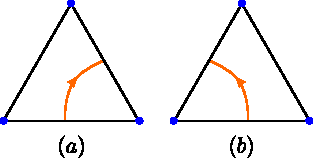
\includegraphics[width=2.1in]{figures/mono-3-crop.pdf}
\caption{右转与左转，由简单的矩阵给出。}\label{fig:mono-3}
\end{minipage}\hspace{0.4cm}
\begin{minipage}[b]{0.45\linewidth}
\centering 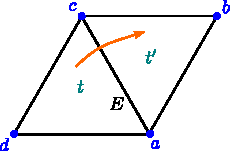
\includegraphics[width=1.6in]{figures/mono-2-crop.pdf}
\caption{穿过三角形 $t$ 与 $t'$ 之间的边 $E$。}\label{fig:mono-2}
\end{minipage}
\end{figure}

现在，$s_i,s_j,s_k$ 起初只定义在顶点 $i,j,k$ 的割缝邻域中。我们可以把它们延拓得在整个三角形 $t$ 上单值；而且事实上还能继续延拓到路径 $P$ 接下来所遇的三角形 $t'$ 中，使它们在更大的区域 $t\cup t'$ 上有定义且单值；如此继续，只要该区域保持单连通即可。我们将通过计算路径 $P$ 沿途从一组这样的基到另一组的变换，来算出单值矩阵。所需的基变换有两类。若路径经由一条边 $E$ 进入三角形 $t$、又经由边 $E'$ 离开三角形 $t$，我们就需要矩阵 $M_E^{E'}(t)$，它给出三角形 $t$ 内与两条边相联系的两组基之间的基变换，如图 85 所示% TODO 合稿改 \ref{fig:mono-3}
。另一方面，若路径经由一条边 $E$ 从三角形 $t$ 穿到三角形 $t'$，我们就需要两组不同基之间的变换 $M_t^{t'}(E)$，如图 86 所示% TODO 合稿改 \ref{fig:mono-2}
。

我们先说明如何计算 $M_E^{E'}(t)$。在三角形 $t$ 内有简单的关系
\begin{equation}
s_1 (s_2 \wedge s_3) + s_2 (s_3 \wedge s_1)+ s_3 (s_1 \wedge s_2)=0
\end{equation}
利用这一关系，基变换
\begin{equation}
\CB(E,t) = \CB(E',t) M_{E}^{E'}(t)
\end{equation}
便可轻易算出，其中
\begin{equation}\label{eq:left-right-turn}
M_{E}^{E'}(t) = \begin{cases} \begin{pmatrix} 0 & -1 \\ 1 & -1 \end{pmatrix}&
\langle E,E'\rangle = +1 \\ \begin{pmatrix} -1 & 1 \\ -1 & 0 \end{pmatrix}&
\langle E,E'\rangle = -1 \end{cases}
\end{equation}
注意 $\det M_{E}^{E'}(t)=1$，并且 $\langle E,E'\rangle=1$ 的情形对应于\emph{右}转，即图 85 中标为 a) 的那一种% TODO 合稿改 \ref{fig:mono-3}
。还要注意：右转矩阵是左转矩阵的逆。

另一方面，若 $t\cup t'$ 拼成一个四边形 $Q_E$，其顶点按逆时针顺序为 $a,b,c,d$（于是 $t$ 的顶点为 $acd$、$t'$ 的顶点为 $abc$，而 $E$ 就是边 $ac$，如图 86 所示% TODO 合稿改 \ref{fig:mono-2}
），则
\begin{equation}
\CB(E,t') = \CB(E,t)\begin{pmatrix} 0 & \frac{s_b \wedge s_c}{s_c \wedge
s_d} \\ \frac{s_a \wedge s_b}{s_d \wedge s_a} & 0 \end{pmatrix}
\end{equation}
从而
\begin{equation}\label{eq:M-edge-matrix}
M_{t}^{t'}(E) =\frac{s_b \wedge s_c}{s_c \wedge s_d} \begin{pmatrix}
0 & 1 \\ - \CX_E^T & 0 \end{pmatrix}
\end{equation}
在下文的论证中，把上式记作
\begin{equation}
\hat M_{t}^{t'}(E) :=
\begin{pmatrix} 0 & 1 \\ - \CX_E^T & 0 \end{pmatrix}
\end{equation}
会很方便。注意 $\det \hat M_{t}^{t'}(E) = \CX_E^T$。

\insfig{3.8in}{mono-1}{我们沿橙色路径、通过在相继各三角形内部及其之间的逐次基变换，来计算单值（矩阵）。}

现在考虑如图 87 那样穿过若干三角形的一条路径% TODO 合稿改 \ref{fig:mono-1}
。把基 $\CB(E_1,t_1)$ 沿一条开路平行移动，所得基 $\tilde\CB(E_1,t_1)$ 在该开路所经各相继三角形拼成的单连通区域上处处单值；于是在该开路的末三角形 $t_f$ 中有如下关系：
\begin{equation}
\CB(E_f, t_f) =\tilde\CB(E_1,t_1) M_{E_1}^{E_2}(t_1)
M_{t_1}^{t_2}(E_2) M_{E_2}^{E_3}(t_2) \cdots M_{t_{f-1}}^{t_f}(E_f)
\end{equation}
现在设路径闭合，即取 $t_f=t_1$、$E_f = E_1$。此时 $\tilde\CB(E_1,t_1) = \CB(E_1,t_1) \cdot \CU(P)$，其中 $\CU(P)$ 是闭路径 $P$ 的单值矩阵在基 $\CB(E_1,t_1)$ 下的表示。由于该基只在相差标度的意义下确定，而 $\CU(P)$ 在任何基变换下只作共轭，可见 $\CU(P)$ 是一个确定的 $SL(2,\IC)$ 矩阵，它与为构造 $\CB(E_1,t_1)$ 而对 $s_i,s_j,s_k$ 所作的标度选取无关。因此 $\CU^{-1}$ 就是上述那些 $M$-矩阵的乘积。然而，由于方程 \eqref{eq:M-edge-matrix} 中的标量前因子 $\frac{s_b \wedge s_c}{s_c \wedge s_d}$，单值矩阵 $\CU(P)$ 能否用边坐标表出，并不显然。不过我们可以用下面这个技巧。矩阵 $\CU(P)^{-1}$ 在相差一个标量因子的意义下，与把各因子 $M_{t}^{t'}(E)$ 换成 $\hat M_{t}^{t'}(E)$ 之后所得的乘积相同。也就是说，有
\begin{equation}
\CU(P)^{-1} = \kappa M_{E_1}^{E_2}(t_1) \hat M_{t_1}^{t_2}(E_2)
M_{E_2}^{E_3}(t_2) \cdots \hat M_{t_{f-1}}^{t_f}(E_f)
\end{equation}
其中 $\kappa$ 是某个标量因子。取行列式即可定出 $\kappa^2$：
\begin{equation}
\kappa^{-2}  =   \CX_{E_2}^T \cdots \CX_{E_f}^T
\end{equation}
于是 $\kappa$ 含有沿路径 $P$ 所遇各边之 $\CX_E^T$ 连乘积的平方根。为定义这个平方根，我们可以援引某种非阿贝尔版本的斯托克斯定理：若 $C$ 是带穿刺点的 $\IC\IP^1$，则闭曲线 $P$ 围出一块区域 $\CR$；而由第 5.2 节所述结果% TODO 合稿改 \ref{sec:monodromies}
的推广，有
\begin{equation}
  \CX_{E_2}^T \cdots \CX_{E_f}^T \prod_{E\in {\rm
Int}(\CR)} (\CX_E^T)^2 = \prod_{v\in {\rm Int}(\CR)} (\mu_v)^2.
\end{equation}
这个公式使我们能以典范的方式选取平方根，即
\begin{equation}
\kappa = (  \CX_{E_2}^T \cdots \CX_{E_f}^T)^{-1/2} =
\frac{\prod_{E\in {\rm Int}(\CR)} \CX_E^T}{\prod_{v\in {\rm
Int}(\CR)} \mu_v}.
\end{equation}

最后我们作几点评论：

\begin{enumerate}

\item 在上面的讨论中，我们假定了所有三角形都非退化。如果出现如图 19 那样的退化构形% TODO 合稿改 \ref{fig:degenerate-face}
，我们就把边 $E$ 视为加倍的。于是，在中心顶点处取装饰 $s_1$、在外侧顶点处取装饰 $s_2$，并在上述构造中使用三个截面 $s_1,Ms_2,s_2$，其中 $M$ 是绕中心顶点的顺时针单值（变换）。特别地，我们把 $E$ 看成具有「两侧」：左侧的基为 $\CB_{\rm left} = \{ s_1 (M s_2 \wedge s_2), M s_2 ( s_2 \wedge s_1) \}$，右侧的基为 $\CB_{\rm right} = \{ s_2 (s_1 \wedge M s_2),s_1 (M s_2 \wedge s_2) \}$。对于绕着边 $E$ 而行的路径，我们用边到边的变换把这两组基联系起来。对于从左穿到右、经过边 $E$ 的路径，我们用 $M^{-1}$ 把 $\CB_{\rm left}$ 沿该边解析延拓，得到如下基变换：
\begin{equation}
\CB_{\rm right} = \tilde \CB_{\rm left} \begin{pmatrix} 0 & \mu \\ -
\mu^{-1} & 0 \end{pmatrix}.
\end{equation}
对图 20 中那个外侧的退化三角形，也有类似的说明% TODO 合稿改 \ref{fig:degenerate-quadrilateral}
。

\item 要把这一结果推广到 $C$ 为亏格更高的带穿刺点曲面的情形，我们需要选定一组平方根 $(\CX_{E_2}^T \cdots \CX_{E_f}^T)^{-1/2}$。只需对非边界闭链的一组基给出这些平方根即可；因此，这样一组选取的全体构成 $H_1(\bar C, \IZ_2)$ 的一个挠子。

\item 单值矩阵的矩阵元显然是 $\CX_{E}^T$ 的\emph{多项式}（再除以若干 $\mu_v$ 因子）；特别地，闭路径 $P$ 的单值矩阵之迹可以写成
\begin{equation}\label{eq:UV-IR-monodromy}
{\Tr}\ \CU(P) = \sum_\gamma a_\gamma(P) \CX_\gamma.
\end{equation}
几何系数 $a_\gamma(P)$ 依赖于三角剖分，因而特别地依赖于 $\vartheta$。注意 \eqref{eq:UV-IR-monodromy} 的左端与 $\vartheta$ 无关，所以 $a_{\gamma}(P)$ 与 $\CX_\gamma^\vartheta$ 的间断必须互相抵消。在五维 Yang--Mills 理论中，${\Tr}\ \CU(P)$ 是沿 $C$ 中路径 $P$ 的、关于 $\CA$ 的超对称 Wilson 线算符的真空期望值。显然，它源自非阿贝尔六维 $(2,0)$ 理论中的一个面算符，该面算符缠绕 $C$ 中某个一维闭链与 $S^1_R$ 的乘积。这表示紫外四维规范理论中的一个线算符。视闭链 $\gamma$ 的不同，这个线算符可以是四维规范场的 Wilson 圈算符、一个 't Hooft 算符，或更一般的 Wilson--'t Hooft 算符。有鉴于此，我们把方程 \eqref{eq:UV-IR-monodromy} 解读为如下关系：它把紫外理论中定义的线算符，与这一线算符在另一组线算符基下的分解联系起来，而后者携带红外阿贝尔理论的量子数。的确，$\CX_{\gamma}$ 就是绕 $S^1_R$ 缠绕的线算符的期望值，这些线算符定义在红外的四维 $\CN=2$ 理论中（等价地说，是红外阿贝尔 $(2,0)$ 理论在 $\IR^{1,2} \times S^1_R\times \Sigma$ 上的面算符）。

存在一个依赖于 $\zeta$ 的幂零超对称算符 $Q_\zeta$，它湮灭这些算符；因此它们是超对称 't Hooft--Wilson 线算符的类似物，与 \cite{Maldacena:1998im,Rey:1998ik,geom-lang-n4} 中所讨论的那些相仿。按此解释，方程 \eqref{eq:UV-IR-monodromy} 编码了一些有趣的物理，我们希望另文讨论。

\item 关于 $SL(2,\IC)$ 联络的模空间与 $PSL(2,\IC)$ 联络的模空间之间的区别，有一点微妙之处需要说明。本文考虑的是 $C$ 上平凡化的 $SL(2,\IC)$ 主丛上的联络，或它在对中心取商后所得的平凡化 $PSL(2,\IC)$ 丛上的联络。这两种丛上的联络之间存在一一对应。然而，存在一些 $PSL(2,\IC)$ 规范变换不能提升为 $SL(2,\IC)$ 规范变换，因此 $SL(2,\IC)$ 联络的模空间是 $PSL(2,\IC)$ 联络的模空间的一个离散覆盖。$\CX_{\gamma}$ 定义在 $PSL(2,\IC)$ 联络的商模空间上，并可拉回到 $SL(2,\IC)$ 联络的模空间上。如果我们认为模空间是由单值本征值 $\mu_i$ 的指定（而不只是 $\mu_i^2$ 的指定）所确定的，那么当 $C = \IC \IP^1$ 时，$\CX_E^T$ 就唯一地确定了一个模 $SL(2,\IC)$ 规范不变的平坦 $SL(2,\IC)$ 联络。对于亏格更高的 $C$，即便指定了 $\mu_i$，$\CX_E^T$ 也不足以完全分辨 $SL(2,\IC)$ 联络模空间上的点：要由 $\CX_E^T$ 确定联络，我们还需要指定那组平方根 $(\CX_{E_2}^T \cdots \CX_{E_f}^T)^{-1/2}$。这些选取的存在引出一个问题：$\IR^3 \times S^1$ 上四维规范理论「正确」的模空间究竟是什么？它应当是 $SL(2,\IC)$ 联络的模空间、$PSL(2,\IC)$ 联络的模空间，还是 $PSL(2,\IC)$ 联络模空间的某个中间覆盖？有趣的是，定义相应的四维规范理论本身也涉及一个离散选取，而它也许正对应于上述含混之处。如 \cite{Gaiotto:2009we} 所述，相应的四维规范理论是若干 $SU(2)$ 规范群构成的广义箭图。规范群中心的一个子群 $\CC$ 在物质场上平凡地作用，于是我们有权把规范群对 $\CC$ 的任一子群取商。与众所周知的 $\CN=2^*$ $SU(2)$ 规范理论（它联系于带一个穿刺点的环面上的 Hitchin 方程）作比较，应当足以建立完整的对应词典；但我们不在此深究此事。

\end{enumerate}

\begin{yizhu}
原文在 (A.14) 处写 $\CX_\gamma$（不带任何上标），而同一段后文又写成 $\CX_\gamma^\vartheta$；按第 7 节% TODO 合稿改 \ref{sec:darboux-coordinates}
的定义，前者即后者。译文两处均照抄原文记号，未作统一。
\end{yizhu}
